
\section{Deployment Planning}
\label{sec:planning}

The deployment planning is a online part of the presented approach. It is executed in the target environment. It is conducted autonomously, using a metamodel and algorithm to come up with a deployment plan.

\begin{figure}[!htb]
  \centering
  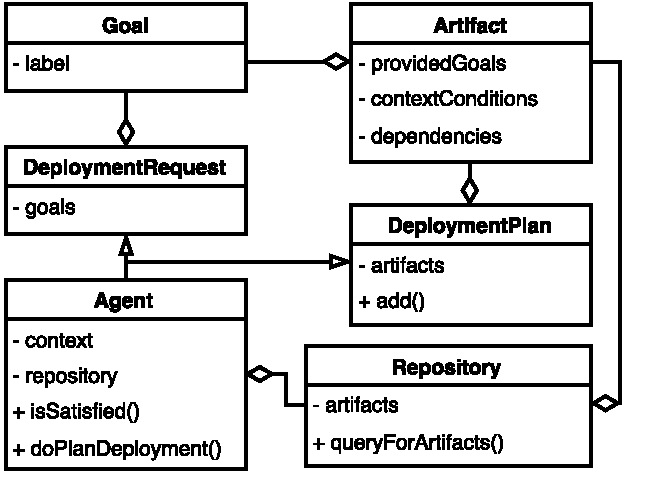
\includegraphics[width=0.95\linewidth]{metamodel}
  \caption{The Goalp Deployment metamodel}
  \label{fig:metamodel}
\end{figure}

Figure~\ref{fig:metamodel} presents the metamodel used. Artifact is the central entity at deployment level. As described in the section~\ref{sec_artifacts}, artifacts has \emph{provided goals}, \emph{context conditions}, and \emph{dependencies}.
Artifacts \emph{provided goals} and \emph{dependencies} create relations of dependency between artifacts, so that an artifact that has a goal dependency is dependent on an artifact that provides that goal. % However, this dependency is loose. An artifact do not depend on one specific other artifact, but instead, on any artifact that provides a goal.

An \emph{agent} can accept deployment requests, action that should trigger the deployment planning. An agent knows a \emph{respository} where it looks for artifacts.
A \emph{repository} has a set of artifacts that it can be queried about by the \emph{queryForArtifacts} method. The method \emph{queryForArtifacts} receives a Goal as argument and return all artifacts in the repository that provide that Goal. An \emph{agent} can verify artifacts \emph{context conditions} satisfaction against its own context by \emph{isSatisfied} method.

The \emph{Deployment Request} is a set of goals that an external entity sent to an agent, requesting it to plan a deployment. The \emph{Deployment Plan} is generated as a result of agent \emph{doPlanDeployment}. The \emph{Deployment Plan} is a set of artifacts that makes the goals specified in the \emph{Deployment Request} achievable.

Note that components do not appear here in this model. Components are architectural units that are packaged into artifacts. The components definitions are mapped and developed by the architect/developer, offline.  And is instantiated and bind by the platform, online. But, it do not appear directly at deployment reasoning, as the abstraction concept at deployment is the artifact.

Artifacts are \emph{deployable} for an agent if all its context conditions and dependencies are satisfiable.
Goals are \emph{achievable} if artifacts that provide that goal are deployable, so there is a \emph{deployment plan} that is able to satisfy this goal.

% \begin{figure}[!htb]
%   \centering
%   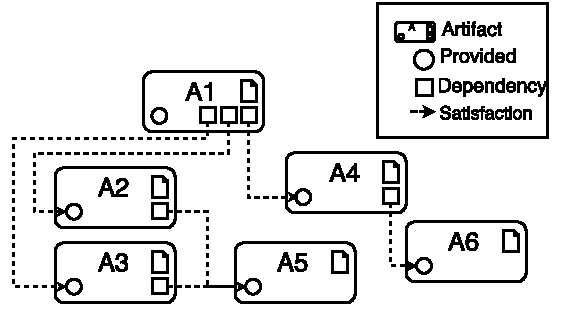
\includegraphics[width=.6\linewidth]{dependency_graph}
%   \caption{Dependency Graph}
% \label{fig:dependency_graph}
% \end{figure}

\subsection{Planning Method}

To come up with a deployment plan for a given a given deployment request and context we present the Algorithm~\ref{plan_method}. It implements the \emph{Agent}'s \emph{doPlanDeployment} method (Figure~\ref{fig:metamodel}).

\begin{algorithm}
 \KwIn{DeploymentRequest request}
 \KwResult{DeploymentPlan plan}
  var resultingPlan $\leftarrow$ new DeploymentPlan() \;

  \ForEach{Goal selectedGoal in goals}{
    var subPlan $\leftarrow$ new DeploymentPlan() \;

    var artifacts $\leftarrow$ repository.
    \\queryForArtifacts(selectedGoal) \;

    \ForEach{Artifact artifact in artifacts}{
     	var contextSatisfaction $\leftarrow$ \\
      isSatisfied(artifact.contextConditions)\;

      \If{contextSatisfaction}{
        var plan $\leftarrow$ new DeploymentPlan ()\;

        plan.add(artifact)\;

        \If{artifact.dependencies == EMPTY}{
          subPlan.add(plan)\;

          break\;
        }\Else{
          var depPlan  $\leftarrow$ doPlanDeployment (artifact.dependencies)\;

          \If{depPlan != NULL}{
          plan.add(depPlan)\;

          subPlan.add(plan)\;

          break\;
          }
        }
      }
    }
    \If{subPlan != EMPTY}{
      resultingPlan.add(subPlan)\;

    }\Else{

      \Return{NULL}
    }
  }
  \Return{resultingPlan}

  \caption{doPlanDeployment (List goals)}
  \label{plan_method}
\end{algorithm}

The Algorithm~\ref{plan_method} works as follows: it receives as parameter as deployment request, which contains a list of goals. For each goal in the list, it queries the repository for artifacts that provides this goals (line 4). The repository returns a list of artifacts. For each artifact the algorithm looks for a sub plan with this artifact (line 5-21). First, the context conditions are verified (line 6). If the context is satisfied (line 7),
then a new plan is created with the artifact (line 8-9). If the list of dependencies of the artifact in empty (line 10), them the new plan is added to the sub plan (line 11). Else, if the artifact has a not empty set of dependencies, the algorithm is recursively called for this dependencies. If the results of the recursive call is not NULL (line 15), the resulting plan is added to the new plan and the plan is added to the sub plan (line 16-17).
In both cases that a new plan is added to a sub plan, the look for a deployment plan that satisfy the selected goal is over and the inner for loop is broken (line 12 and 19) and them the sub plan is added to the resulting plan (line 25).
Otherwise, if the context conditions evaluation (line 6) returns FALSE or the recursive call returns NULL, this artifact can not be deployed. The loops continues and others artifacts will be tried. The algorithm tries to come up with a sup plan for the selected goal with another artifact that provides this goal. If after all tries the sub plan is EMPTY (line 27), the deployment for the selected goal is not possible, and the algorithm returns NULL (line 28). Note that the algorithm will return NULL if for any of the goals in the request it is not possible to come up with a plan. Otherwise, the algorithm will return a valid plan.

It could be the case that there are more then one possible valid plan. But this algorithm will return the first one found.  We let for future works the investigation of approaches to come up with the best alternative plan in case that more then one is valid.

\subsection{Verifying a Plan}
\label{verify_plan}

A deployment plan, is valid for a given context if: (i) for each artifact in the plan, for the current context, all context conditions hold.
(ii) for each artifact, for all its dependencies, there is at least one artifact in the plan that provides it (the dependency).

A deployment plan satisfy a deployment request if it valid, and (iii) for each goal, in the deployment request, there is at least one artifact that provides this goal.

Being so, we can verify if a deployment plan satisfy a deployment request by executing the following steps, that verifies the properties (i), (ii) and (iii):

\begin{itemize}
  \item Check if for all selected artifacts, all context conditions are met.
  \item Check if for all selected artifacts, the dependencies are within the deployment plan.
  \item Check if for all goals in the deployment request there are at least one artifacts that declare this goal and one that implements this goal.
\end{itemize}

\subsection{Deployment Execution}
\label{sec:planning}

The last step of the approach is the deployment execution. The deployment execution involves (i) coping the artifacts present in the deployment plan from the repository to the target environment. And (ii) binding the components present into these artifacts, creating the application architecture.

To bind components, the Dependency Injection design pattern can be used. The basic idea of the Dependency Injection, is to have a separate object, an assembler, that wires together client and server components at runtime\cite{fowler_inversion_2004}. The client refers to a component that uses another component (a service) through an interface. The assembler looks for an available service (implementation of the the interface), instantiates it, and wires it into the client object.
